\documentclass{report}
\usepackage{graphicx}
\usepackage{url}
\usepackage{multirow}
\usepackage{listings}
\usepackage{verbatim}
\usepackage[hybrid,pipeTables]{markdown}
\usepackage{longtable}
\usepackage{booktabs}
\usepackage{adjustbox}

\lstset{
basicstyle=\small\ttfamily,
columns=flexible,
breaklines=true
}

\author{
    \begin{tabular}{l l}
        \textbf{Submitted By} & \textbf{Sumbitted To} \\
        Aadarsha Dhakal & Asst.Prof.Rajani Chulyado \\
        \multirow{2}{*}{Roll No: 12}  & Department of Computer \\
                                      & Science and Engineering
    \end{tabular}
}
\title{

\includegraphics[scale=1]{kulogo}\\[1cm]
\LARGE{KATHMANDU UNIVERSITY}\\
\large{\textsc{Department of Computer Science and Engineering}}\\[1cm]
\textsc{\large Database Management System}\\
\large{COMP 232}\\[2cm]
\hrule
\vspace{0.5cm}
Lab 2 Report
\vspace{0.5cm}
\hrule
}
\date{
    \vspace{0.5cm}
    {Date: 20-02-2022}
}


\begin{document}
\maketitle
\tableofcontents
\listoffigures
\newpage

\begin{figure}
\centering
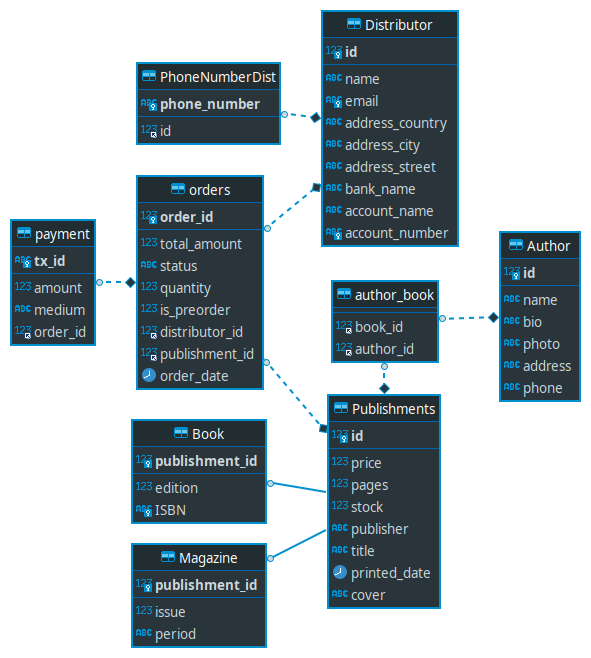
\includegraphics[width=\textwidth]{erdiagram}
\caption{Database ER Diagram}
\end{figure}

\chapter{DDL Scripts}
\section{Creating the tables}
\begin{verse}
    \lstinputlisting{creating_tables.sql}
\end{verse}
\section{Populating data}
\begin{verse}
    \lstinputlisting{populating_data.sql}
\end{verse}

\chapter{Queries}

\section{Find the name of all published books.}

\begin{lstlisting}
    SELECT * from Book b INNER JOIN Publishments p ON b.publishment_id = p.id
\end{lstlisting}
\vspace{0.5cm}
\textbf{Relational Algebra :} \[  \rho_p(Publishments) \bowtie_{b.publishment\_id = p.id}  \rho_b(Book)   \]
\paragraph{Description: }
Creates innter join of table Publishments and Book.

\paragraph{Output: }

\begin{longtable}[]{@{}llllll@{}}
\toprule
publishment\_id & edition & ISBN & id & price & pages \\
\midrule
\endhead
1 & 1.0 & 1234567 & 1 & 500.0 & 800 \\
2 & 3.0 & 6585645 & 2 & 12050.0 & 100 \\
\bottomrule
\end{longtable}


\section{Find the name of all books published before 2000.}

\begin{lstlisting}
   SELECT  title from Book b INNER JOIN Publishments p ON b.publishment_id =p.id WHERE printed_date < '2000-01-01'
\end{lstlisting}
\vspace{0.5cm}
\textbf{Relational Algebra :} \[ \prod_{title}(\sigma_{printed\_date < '2000-01-01'}( \rho_p(Publishments) \bowtie_{b.publishment\_id = p.id}  \rho_b(Book)) ) \]
\paragraph{Description: }
Selects title from the inner join of Book and Publiushments where the printed\_date is before 2020. 

\paragraph{Output: }
\begin{longtable}[]{@{}l@{}}
\toprule
title \\
\midrule
\endhead
Auna Ratnamala \\
\bottomrule
\end{longtable}



\section{Get the details of the books written by a particular author.}
\begin{lstlisting}
   SELECT  * from author_book ab INNER JOIN Author a ON ab.author_id = a.id INNER JOIN Book b ON ab.book_id = b.publishment_id  INNER JOIN Publishments p ON b.publishment_id =p.id WHERE name="Aadarsha Dhakal"
\end{lstlisting}
\vspace{0.5cm}
\textbf{Relational Algebra :} \[ \sigma_{name = "Aadarsha Dhakal"}  ( \rho_{ab}(author\_book) \bowtie_{ab.author\_id = a.id} \rho_a(Author)\]\[ \bowtie_{ab.book\_id = b.publishment_id} \rho_b(Book) \bowtie_{b.publishment\_id = p.id} \rho_p(Publishments) ) \]
\paragraph{Description: }
Creates Join of author\_book table, Author table and Book table and Publiushments table and find the tuples where name is the 'Aadarsha Dhakal'.

\paragraph{Output: }

\begin{longtable}[]{@{}llllll@{}}
\toprule
book\_id & author\_id & name & phone &
ISBN & price \\
\midrule
\endhead
1 & 1 & Aadarsha Dhakal
& 9869698962 & 1234567 & 500.0 \\
\bottomrule
\end{longtable}



\section{Find the name of all weekly publications. }
\begin{lstlisting}
   SELECT title from Publishments p INNER JOIN Magazine m ON p.id = m.publishment_id WHERE period='Weekly'
\end{lstlisting}
\vspace{0.5cm}
\textbf{Relational Algebra :} \[ \prod_{title}( \sigma_{period='Weekly'}  ( \rho_p(Publishments) \bowtie_{p.id = m.publishment_id}  \rho_m(Magazine)))   \]
\paragraph{Description: }
Selects title from innter join of table Publishments and Magazine where period = 'Weekly'.

\paragraph{Output: }

\begin{longtable}[]{@{}l@{}}
\toprule
title \\
\midrule
\endhead
Times India Magazine \\
\bottomrule
\end{longtable}




\section{Find the name of pre-ordered books.}

\begin{lstlisting}
    SELECT  title FROM orders o INNER JOIN Publishments p ON o.publishment_id =p.id WHERE is_preorder = True
\end{lstlisting}
\vspace{0.5cm}
\textbf{Relational Algebra :} \[ \prod_{title}( \sigma_{is\_preorder = True} (   \rho_o(orders) \bowtie_{o.publishment\_id = p.id}  \rho_p(Publishments)))   \]
\paragraph{Description: }
Selects title from inner join of table Publishments and orders where order's publishment\_id is equal to publishment's id.

\paragraph{Output: }

\begin{longtable}[]{@{}l@{}}
\toprule
title \\
\midrule
\endhead
Auna Ratnamala \\
\bottomrule
\end{longtable}




\section{Get the details of all publications with the name starting with an 'A'.}

\begin{lstlisting}
    SELECT * FROM Publishments p WHERE title LIKE 'A%'
\end{lstlisting}
\vspace{0.5cm}
\textbf{Relational Algebra :} \[ \sigma_{title\ LIKE\ 'A\%'}  \rho_p(Publishments)  \]
\paragraph{Description: }
Retrives tuples from Publishments table where title starts with letter 'A'.

\paragraph{Output: }

\begin{longtable}[]{@{}lllll@{}}
\toprule
id & price & publisher & title & printed\_date\\
\midrule
\endhead
1 & 500.0 & Manjari Publications & Auna Ratnamala & 1922-02-15 \\
\bottomrule
\end{longtable}



\section{Find all the orders for a particular book. The result must be sorted based on the order date. }

\begin{lstlisting}
    SELECT * FROM  orders o INNER JOIN Publishments p ON o.publishment_id = p.id INNER JOIN Book b ON p.id = b.publishment_id ORDER BY order_date DESC
\end{lstlisting}
\vspace{0.5cm}
\textbf{Relational Algebra :} \[ \tau_{order\_date\ \downarrow} ( \rho_p(Publishments) \bowtie_{o.publishment\_id = p.id} \rho_o(orders) \bowtie_{p.id = b.publishment\_id} \rho_b(Book) )  \]
\paragraph{Description: }
Retrives tuples from INNER JOIN of orders table, Publishments table and Book table and are ordered descendingly by order\_date.

\paragraph{Output: }

\begin{longtable}[]{@{}llllll@{}}
\toprule
order\_id & total\_amount & quantity &
order\_date &
title &
ISBN \\
\midrule
\endhead
2 & 12050.0 & 1 & 2022-02-15 &
University Physics
& 6585645 \\
1 & 2000.0 & 4 & 1980-12-17 &
Auna Ratnamala
& 1234567 \\
\bottomrule
\end{longtable}




\end{document}
